\documentclass[12pt]{article}
\usepackage{lingmacros}
\usepackage{tree-dvips}
\usepackage{graphicx}
\usepackage{float}
\begin{document}

\section*{Breakdown of DataStructures}

\subsection*{Comparison of sorting algorithms on each, vector, linkedlist, and hashtable data structures.\\}


\small We will be comparing the following three sorting algorithms based on their completion in seconds:\\

\begin{itemize}
	\item MergeSort
	\item HeapSort
	\item QuickSort\\\\
\end{itemize}

\small This experiment was conducted with the same data with a length of 12023 items. This data will first be loaded into the data structure before performing a sorting algorithm on the data. This process will be continued for each algorithm and data structure.\\

\small The data holds bid information, this data is originally stored in a .CSV file. its contains 20 different columns but for this program we will be sorting based on the auction id. The auction id is a 5 digit number that is unique.

\subsection*{\small Graphical Overview}


\begin{figure}[H]
	\begin{center}
		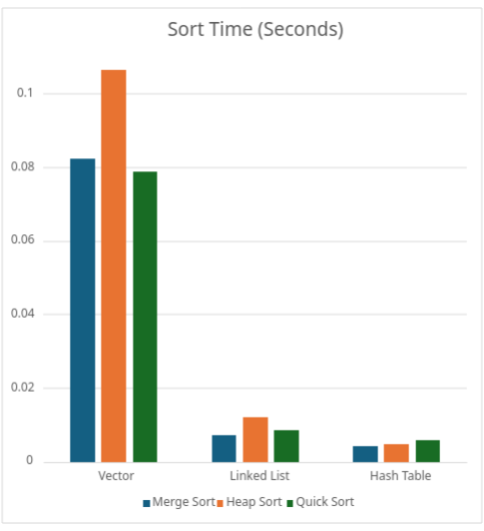
\includegraphics[scale=0.5]{SortTime.png}
	\end{center}
\end{figure}




\begin{enumerate}
	\item \textbf{Vector}
		  \begin{itemize}
		  	\item Merge Sort: 0.0823 seconds
		  	\item Heap Sort: 0.1065 seconds
		  	\item Quick Sort: 0.0789 seconds
		  \end{itemize}
	\item \textbf{LinkedList}
		  \begin{itemize}
		  	\item Merge Sort: 0.0073 seconds
		  	\item Heap Sort: 0.012 seconds
		  	\item Quick Sort: 0.0086 seconds
		  \end{itemize}
	\item \textbf{HashTable}
		  \begin{itemize}
		  	\item Merge Sort: 0.00423 seconds
		  	\item Heap Sort: 0.0049 seconds
		  	\item Quick Sort: 0.006 seconds
		  \end{itemize}
\end{enumerate}

\subsection*{Summarization}

\begin{itemize}
	\item \textbf{Vector} From the data, we can confirm that the vector data structure had the slowest sorting times. The slowest sorting algorithm was the heap sort with an average time of 0.1065.
	\item \textbf{LinkedList} The linkedlist is significantly faster than the vector but still slower than the hashtable. The linked list is in most cases about 10 times quicker than the vector data structure.
	\item \textbf{HashTable} The hashtable consistently performed the sorting algorithms the quickest. The fasted sorting algorithm on average is the merge sort with an average time of 0.00423. On average the hash table was able to sort about twice as fast when compared to the linkedlist.
\end{itemize}

\end{document}